\documentclass[5p,times,twocolumn]{elsarticle}

\usepackage{amsmath,amssymb}
\usepackage{graphicx}
\usepackage{booktabs}
\usepackage{listings}
\usepackage{xcolor}
\usepackage[hidelinks]{hyperref}

\lstset{
  language=Python,
  basicstyle=\ttfamily\scriptsize,
  keywordstyle=\color{blue!60!black},
  commentstyle=\color{black!55},
  stringstyle=\color{green!40!black},
  frame=lines,
  columns=fullflexible,
  keepspaces=true,
  aboveskip=4pt,
  belowskip=2pt,
}

\newcommand{\iDEA}{\textsc{iDEA}}
\newcommand{\vext}{v_\mathrm{ext}}
\newcommand{\vks}{v_\mathrm{KS}}
\newcommand{\vxc}{v_\mathrm{xc}}
\newcommand{\vH}{v_\mathrm{H}}

% Numerical results generated by scripts/make_figures.py
% Generated by paper/scripts/make_figures.py -- do not edit by hand.
\newcommand{\numESinglet}{0.779893}
\newcommand{\numETriplet}{0.936028}
\newcommand{\numEexact}{-1.3413}
\newcommand{\numEhartree}{-0.8852}
\newcommand{\numEhartreefock}{-1.3388}
\newcommand{\numEhybrid}{-1.3379}
\newcommand{\numElda}{-1.3348}
\newcommand{\numEnoninteracting}{-1.6388}
\newcommand{\numEsinglet}{-1.7162}
\newcommand{\numconvEA}{-1.34519}
\newcommand{\numconvEB}{-1.34131}
\newcommand{\numconvEC}{-1.33995}
\newcommand{\numconvdxA}{0.200}
\newcommand{\numconvdxB}{0.133}
\newcommand{\numconvdxC}{0.100}
\newcommand{\numdESinglet}{3.7e-12}
\newcommand{\numdETriplet}{1.6e-12}
\newcommand{\numdnRE}{1.0\times10^{-8}}
\newcommand{\numdnSinglet}{1.1e-11}
\newcommand{\numdnTD}{2.0e-13}
\newcommand{\numdnTriplet}{4.0e-12}
\newcommand{\numdnhartree}{0.654}
\newcommand{\numdnhartreefock}{0.005}
\newcommand{\numdnhybrid}{0.009}
\newcommand{\numdnlda}{0.050}
\newcommand{\numdnnoninteracting}{0.418}
\newcommand{\numfigdx}{0.133}
\newcommand{\numfignx}{181}
\newcommand{\numgridMaxThree}{40}
\newcommand{\numgridMaxTwo}{220}
\newcommand{\numhptErr}{4.0e-08}
\newcommand{\numhptGap}{0.25000004}
\newcommand{\numhptOmega}{0.25}
\newcommand{\numhptdAmp}{0.53}
\newcommand{\numhptdDt}{0.05}
\newcommand{\numhptdDtHalf}{0.025}
\newcommand{\numhptdErr}{4.0e-03}
\newcommand{\numhptdErrHalf}{2.0e-03}
\newcommand{\numinfSinglet}{5.8e-15}
\newcommand{\numinfTriplet}{3.7e-14}
\newcommand{\numipSinglet}{0.577}
\newcommand{\numipTriplet}{0.202}
\newcommand{\numnAtEight}{3\times10^{-3}}
\newcommand{\numnAtFour}{7\times10^{-2}}
\newcommand{\numnAtZero}{5\times10^{-1}}
\newcommand{\numtdAmp}{0.94}
\newcommand{\numtdDt}{0.1}
\newcommand{\numtdField}{0.05}
\newcommand{\numtdNx}{121}
\newcommand{\numtdPulse}{1}
\newcommand{\numtdSteps}{1000}
\newcommand{\numtdTime}{67}
\newcommand{\numtdTmax}{100}
\newcommand{\numtimeMaxThree}{20}
\newcommand{\numtimeMaxTwo}{21}
\newcommand{\numvcMax}{0.013}
\newcommand{\numvcMin}{-0.021}
\newcommand{\numvxcAsymEight}{-0.111}
\newcommand{\numvxcAsymFour}{-0.200}
\newcommand{\numvxcAsymZero}{-1.000}
\newcommand{\numvxcExactEight}{-0.133}
\newcommand{\numvxcExactFour}{-0.293}
\newcommand{\numvxcExactZero}{-0.503}
\newcommand{\numvxcLDAEight}{-0.029}
\newcommand{\numvxcLDAFour}{-0.225}
\newcommand{\numvxcLDAZero}{-0.414}


\journal{Computer Physics Communications}

\begin{document}

\begin{frontmatter}

\title{\iDEA: an open-source Python framework for exact many-electron quantum mechanics and density functional theory in one dimension}

\author[york]{Jack Wetherell\corref{cor1}}
\ead{jack.wetherell@gmail.com}
\author[york]{Matt J. P. Hodgson}
\author[york]{Leopold Talirz}
\author[york]{Rex W. Godby}
\cortext[cor1]{Corresponding author.}
\address[york]{Department of Physics and York Centre for Quantum Technologies, University of York, York YO10 5DD, United Kingdom}

\begin{abstract}
We present \iDEA{} (interacting Dynamic Electrons Approach), a free and open-source Python framework for the exact solution of the static and time-dependent many-electron Schr\"odinger equation for finite one-dimensional systems, together with a family of approximate methods (non-interacting, Hartree, Hartree--Fock, local density approximation, hybrid functionals and Kohn--Sham strictly-correlated electrons) that share a common interface. Exact Kohn--Sham, and more generally exact fictitious-system, potentials are obtained by reverse engineering the exact ground-state or time-dependent density. \iDEA{} is designed for reproducibility, interactivity and simplicity. It has been used to provide exact benchmarks for density functional and many-body perturbation theory, to generate training data for machine learning, and to teach many-body quantum physics. We describe the methods and their implementation, validate them against analytic results, and illustrate their use with three examples.
\end{abstract}

\begin{keyword}
exact diagonalisation \sep density functional theory \sep time-dependent DFT \sep exact Kohn--Sham potential \sep reverse engineering \sep one-dimensional model systems
\end{keyword}

\end{frontmatter}

% ---------------------------------------------------------------------------
\section*{Program summary}
\noindent\emph{Program title:} \iDEA{} (interacting Dynamic Electrons Approach)\\
\emph{CPC Library link to program files:} (to be added by Technical Editor)\\
\emph{Developer's repository link:} \url{https://github.com/JackWetherell/iDEA}\\
\emph{Licensing provisions:} GNU General Public License v3.0\\
\emph{Programming language:} Python ($\geq 3.8$)\\
\emph{External routines/libraries:} NumPy~\cite{NumPy}, SciPy~\cite{SciPy}, Matplotlib, tqdm; optionally CuPy~\cite{CuPy} for GPU acceleration.\\
\emph{Nature of problem:} Exact ground, excited and time-dependent many-electron wavefunctions of finite one-dimensional systems with arbitrary external potentials, interactions and spin configurations are needed as reference data against which approximate methods, such as Kohn--Sham density functional theory (DFT), time-dependent DFT and Hartree--Fock theory, can be assessed. The exact Kohn--Sham potential corresponding to a given interacting density is also required.\\
\emph{Solution method:} The many-electron Hamiltonian is represented on a real-space grid using high-order finite differences, and the lowest eigenstates are found by sparse Lanczos diagonalisation followed by explicit antisymmetrisation of the spin-orbital wavefunction. Time propagation uses the action of the matrix exponential. Approximate methods share a self-consistent single-particle framework. Exact Kohn--Sham potentials are found by iteratively inverting the ground-state or time-dependent density.\\
\emph{Additional comments:} Installable via \texttt{pip install iDEA-latest}. Documentation and a tutorial notebook are provided with the source code.

% ---------------------------------------------------------------------------
\section{Introduction}

Approximate electronic-structure methods are routinely assessed against more accurate methods, but in three dimensions exact many-body solutions are unavailable for all but the smallest systems. Finite one-dimensional (1D) model systems offer a practical alternative: with a softened Coulomb interaction~\cite{Javanainen1988} they show many of the qualitative features of real atoms, molecules and materials~\cite{Wagner2012,Baker2015,Helbig2011}, yet the many-electron Schr\"odinger equation can be solved exactly for a few electrons. Exact solutions give access to the quantities that approximate theories try to model, most notably the exact Kohn--Sham (KS) potential of density functional theory (DFT)~\cite{HK1964,KS1965} and its time-dependent counterpart~\cite{RG1984,Maitra2016,Ullrich2012}. These are unknown in general and must be obtained by inverting the exact density~\cite{vanLeeuwen1994,WuYang2003,Jensen2018,Kanungo2019,Shi2022}.

\iDEA{} (interacting Dynamic Electrons Approach) grew out of this programme in the group of R.~W.~Godby at the University of York. Its exact time-dependent solutions and reverse-engineered KS potentials revealed the static and dynamic steps of the exact exchange--correlation (xc) potential~\cite{Ramsden2012,Hodgson2013,Hodgson2016,Hodgson2017}, complementing related studies by others~\cite{Elliott2012,Ruggenthaler2015}. The code has since been used to construct local density approximations (LDAs) from finite systems~\cite{Entwistle2016,Entwistle2018}, and to assess hybrid functionals~\cite{Elmaslmane2018}, the GW approximation~\cite{Wetherell2018}, the nearsightedness of many-body perturbation theory relative to KS DFT~\cite{Wetherell2019}, generalized KS theory~\cite{Hodgson2020PRA}, and exact potentials for the fundamental gap~\cite{Hodgson2021PRA}. It has also generated exact one-body density matrices for machine learning~\cite{Wetherell2020FD,Snyder2012,Li2016}, informed community discussions on excited states and large-scale simulation~\cite{FD2020excited,FD2020largescale}, and been used in teaching.

The current version, \iDEA{}~1.1, is a rewrite of the original research code. It is a pip-installable Python package with a small, uniform interface designed for reproducibility, interactivity (for example in Jupyter notebooks) and simplicity. General-purpose packages either target three-dimensional systems with approximate methods~\cite{Octopus2020,PySCF2020}, treat lattice or second-quantised models~\cite{QuSpin2017,OpenFermion2020}, or invert densities supplied by other codes~\cite{Shi2022}. In contrast, \iDEA{} combines exact real-space many-electron solutions, the standard approximate methods and density inversion, ground state and time dependent, within one consistent framework.

% ---------------------------------------------------------------------------
\section{Methods and implementation}

\paragraph{Systems}
A \texttt{System} is defined by a uniform grid $x_i$ with spacing $\delta x$, an external potential $\vext(x)$, an interaction $v_\mathrm{int}(x,x')$ and a string of electron spins, e.g.\ \texttt{"uud"}. The default interaction is the softened Coulomb interaction $v_\mathrm{int}(x,x')=1/(|x-x'|+1)$ (Hartree atomic units throughout). The kinetic energy $-\tfrac12\,\mathrm{d}^2/\mathrm{d}x^2$ is represented by central finite differences of 3 to 13 points (default 13), and hard-wall boundary conditions are implied at the grid edges.

\paragraph{Exact solution}
For $N$ electrons the spatial Hamiltonian
\begin{equation}
\hat H=\sum_{i=1}^{N}\hat h_i+\sum_{i<j}v_\mathrm{int}(x_i,x_j),\qquad \hat h=-\tfrac12\tfrac{\mathrm{d}^2}{\mathrm{d}x^2}+\vext(x),
\end{equation}
is assembled as a sparse matrix of dimension $N_x^N$. The one-body part is a Kronecker sum, $\sum_i I\otimes\cdots\otimes h\otimes\cdots\otimes I$, and the interaction is diagonal. The lowest eigenpairs are found with the implicitly restarted Lanczos method (ARPACK~\cite{ARPACK} via SciPy~\cite{SciPy}). Each spatial eigenvector $\psi$ is combined with the spin function $\chi$ defined by the spin string, and the antisymmetriser $\sum_P(-1)^P\hat P$ is applied explicitly over all $N!$ permutations of the space--spin coordinates. Spatial states with the wrong exchange symmetry vanish and are discarded, so the $k$th surviving state is the $k$th fermionic eigenstate. Ground and excited states are thus obtained without imposing symmetry on the spatial problem.

Time propagation in the presence of a perturbation $\delta v(x,t)$ uses
$\Psi(t+\delta t)=\exp[-\mathrm{i}\,\delta t\,\hat H(t+\delta t)]\,\Psi(t)$,
where the action of the matrix exponential is evaluated without forming it, using the algorithm of Al-Mohy and Higham~\cite{AlMohy2011}. Optionally, Hamiltonian construction, diagonalisation and propagation run on a GPU through CuPy~\cite{CuPy}. On an NVIDIA RTX 4090 this reduces the two-electron ground-state solve on a 450-point grid from about 260~s on an Intel i9-11900K CPU to about 17~s, and 20 propagation steps on a 300-point grid from 3.3~s to 0.5~s (benchmark scripts in the repository).

\paragraph{Approximate methods}
Non-interacting electrons, Hartree, restricted and unrestricted Hartree--Fock (HF)~\cite{Fock1930}, the LDA, hybrid functionals and Kohn--Sham strictly-correlated electrons (KS-SCE)~\cite{Malet2012,Malet2013,Mirtschink2013,Marie2022} share one self-consistent single-particle solver. For each spin channel the Hamiltonian $h_\sigma[n,\rho_\sigma]$ is diagonalised densely, and the density $n$ and spin-resolved density matrices $\rho_\sigma(x,x')$ are mixed linearly until $\int|n-n_\mathrm{old}|\,\mathrm{d}x$ falls below a tolerance. Each method supplies only its potential, $\vH$, $\vH+v_\mathrm{x}^\mathrm{HF}$, $\vH+\vxc^\mathrm{LDA}$, $\vH+\alpha v_\mathrm{x}^\mathrm{HF}+(1-\alpha)\vxc^\mathrm{LDA}$, or $v_\mathrm{SCE}$, and its total-energy expression. The LDA uses the exchange and correlation energies of the spin-polarised 1D homogeneous electron gas parametrised in Refs.~\cite{Entwistle2016,Entwistle2018}. Excited Slater determinants are obtained by occupying higher orbitals. Time-dependent versions (TDHF, adiabatic LDA, etc.) propagate the occupied orbitals with the same exponential integrator, rebuilding the Hamiltonian from the density and density matrix at each step.

\paragraph{Reverse engineering}
For a target density $n_\mathrm{T}(x)$ and a chosen method, \iDEA{} finds the external potential of the fictitious system that reproduces $n_\mathrm{T}$ by iterating
\begin{equation}
v^{(i+1)}(x)=v^{(i)}(x)+\mu\left[n^{(i)}(x)^{p}-n_\mathrm{T}(x)^{p}\right],
\label{eq:re}
\end{equation}
until $\int|n^{(i)}-n_\mathrm{T}|\,\mathrm{d}x$ is below a tolerance. Here $\mu>0$ and $0<p\le 1$ (default $p=0.1$, which accelerates convergence where the density is small). With the non-interacting method and an exact $n_\mathrm{T}$ this yields the exact KS potential $\vks$, from which $\vxc=\vks-\vext-\vH$. In the time-dependent case the potential at each time step is found by solving for the $\delta v(x,t)$ for which a single propagation step reproduces $n_\mathrm{T}(x,t)$, using Powell's hybrid method in SciPy.

\paragraph{Observables and interface}
The \texttt{observables} module computes densities, density matrices, and Hartree and exchange potentials and energies from many-body states, single-particle states or their time evolution. Every method module exposes the same functions (\texttt{solve}, \texttt{propagate}, \texttt{total\_energy}, \texttt{hamiltonian}), so methods can be swapped or looped over:
\begin{lstlisting}
import numpy as np, iDEA
x = np.linspace(-12, 12, 241)
s = iDEA.system.System(x, -2/(abs(x)+1),
        iDEA.interactions.softened_interaction(x),
        electrons="uu")
gs = iDEA.methods.interacting.solve(s, k=0)
n = iDEA.observables.density(s, state=gs)
for m in iDEA.iterate_sb_methods:   # NI, H, HF, LDA, hybrid
    st = m.solve(s)
    print(m.name, m.total_energy(s, st))
ks = iDEA.reverse_engineering.reverse(
        s, n, iDEA.methods.non_interacting)
v_xc = ks.v_ext - s.v_ext \
       - iDEA.observables.hartree_potential(s, n)
\end{lstlisting}

% ---------------------------------------------------------------------------
\section{Validation}

% Generated by paper/scripts/make_figures.py -- do not edit by hand.
\begin{table}[t]
\centering\footnotesize
\caption{Validation of the exact solver and indicative cost. (a) Two electrons in a harmonic well ($\omega=0.3275$, $N_x=231$, $L=20$) compared with the separated centre-of-mass/relative-coordinate reference on the same grid: absolute energy error, maximum density error and wavefunction infidelity $1-|\langle\Psi_\mathrm{ref}|\Psi\rangle|$. (b) Lowest dipole excitation energy versus the harmonic-potential theorem, and the time-dependent density error over 500 steps. (c) Grid convergence of the ground-state energy of the atom in Fig.~\ref{fig:gs}. (d) Wall time of \texttt{interacting.solve} on 4 CPU cores of the test machine.}
\label{tab:validation}
\begin{tabular}{@{}lll@{}}
\toprule
\multicolumn{3}{@{}l}{(a) Two-electron ground state} \\
 & singlet (\texttt{ud}) & triplet (\texttt{uu}) \\
\midrule
$E$ (Ha) & 0.779893 & 0.936028 \\
$|\Delta E|$ & $3.7\times10^{-12}$ & $1.6\times10^{-12}$ \\
$\max|\Delta n|$ & $1.1\times10^{-11}$ & $4.0\times10^{-12}$ \\
infidelity & $5.8\times10^{-15}$ & $3.7\times10^{-14}$ \\
\midrule
\multicolumn{3}{@{}l}{(b) Excitations and dynamics} \\
$E_1-E_0$ vs $\omega=0.25$ & 0.25000004 & error $4.0\times10^{-8}$ \\
TD density, $\max|\Delta n(x,t)|$ & $2.0\times10^{-13}$ & \\
driven HPT, $\max|\Delta x_\mathrm{cm}|$, $\delta t=0.05$ & $4.0\times10^{-3}$ & (amplitude 0.53) \\
\quad $\delta t=0.025$ & $2.0\times10^{-3}$ & \\
\midrule
\multicolumn{3}{@{}l}{(c) Grid convergence, atom (\texttt{uu})} \\
$\delta x=0.200$ & $E=-1.34519$ & \\
$\delta x=0.133$ & $E=-1.34131$ & \\
$\delta x=0.100$ & $E=-1.33995$ & \\
\midrule
\multicolumn{3}{@{}l}{(d) Ground-state solve time} \\
$N=2$: $N_x$ & \multicolumn{2}{l}{60, 100, 140, 180, 220} \\
\quad time (s) & \multicolumn{2}{l}{0.2, 1.4, 3.4, 9.7, 21.5} \\
$N=3$: $N_x$ & \multicolumn{2}{l}{20, 30, 40} \\
\quad time (s) & \multicolumn{2}{l}{1.1, 6.9, 19.7} \\
\bottomrule
\end{tabular}
\end{table}


The exact solver is tested against a semi-analytic reference (Table~\ref{tab:validation}). For two electrons in a harmonic potential $\vext=\tfrac12\omega^2x^2$ with the softened interaction, the Hamiltonian separates into an analytic centre-of-mass part and a relative-coordinate problem, which is solved on a fine grid. The \iDEA{} energies, densities and wavefunctions agree with this reference for both the spin-singlet (\texttt{ud}) and spin-triplet (\texttt{uu}) states. The harmonic-potential theorem~\cite{Dobson1994} provides a second test. The lowest dipole excitation of interacting electrons in a harmonic well has energy exactly $\omega$, which \iDEA{} reproduces. For time propagation, a single electron displaced in a harmonic well and released undergoes coherent oscillation with an analytic density, which the propagator reproduces at every time step. Because the reference uses the same finite-difference stencil, these tests isolate the many-body construction, eigensolver and antisymmetrisation from discretisation error, which is controlled separately by the grid spacing: for the atom of Fig.~\ref{fig:gs}, whose potential has a cusp at the origin, the ground-state energy changes by about $10^{-3}$~Ha between $\delta x=\numconvdxB$ and $\numconvdxC$ (Table~\ref{tab:validation}c). These tests run in continuous integration, and further tests check the self-consistent methods and a reverse-engineering round trip.

% ---------------------------------------------------------------------------
\section{Examples}

All results below are produced by \texttt{paper/scripts/make\_figures.py} in the repository, which regenerates every figure and number in this paper.

\paragraph{Ground state: comparing approximations}
\begin{figure}[t]
\centering
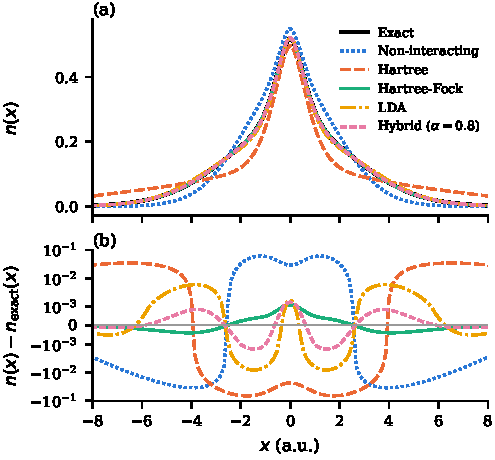
\includegraphics[width=\columnwidth]{figures/fig1_densities.pdf}
\caption{(a) Ground-state density of two spin-polarised electrons in the softened atom $\vext=-2/(|x|+1)$ ($N_x=\numfignx$, $\delta x=\numfigdx$), exact and from each approximate method. (b) Error relative to the exact density.}
\label{fig:gs}
\end{figure}
Figure~\ref{fig:gs} shows two spin-polarised electrons bound by a softened nucleus of charge 2. The exact ground-state energy is $E=\numEexact$~Ha. HF ($\numEhartreefock$~Ha), the LDA ($\numElda$~Ha) and the hybrid ($\numEhybrid$~Ha) are compared with Hartree theory ($\numEhartree$~Ha) and non-interacting electrons ($\numEnoninteracting$~Ha). The integrated density errors $\int|n-n_\mathrm{exact}|\,\mathrm{d}x$ are $\numdnhartreefock$ (HF), $\numdnlda$ (LDA), $\numdnhybrid$ (hybrid) and $\numdnhartree$ (Hartree). The self-interaction contained in the Hartree potential makes its density far too diffuse. The LDA removes much of this error but still slightly over-delocalises the electrons~\cite{MoriSanchez2008}, while HF, which is free of self-interaction for this system, gives the most accurate density. Each method is obtained with the same call, so a comparison like this is a few lines of code.

\paragraph{Exact Kohn--Sham potentials}
\begin{figure}[t]
\centering
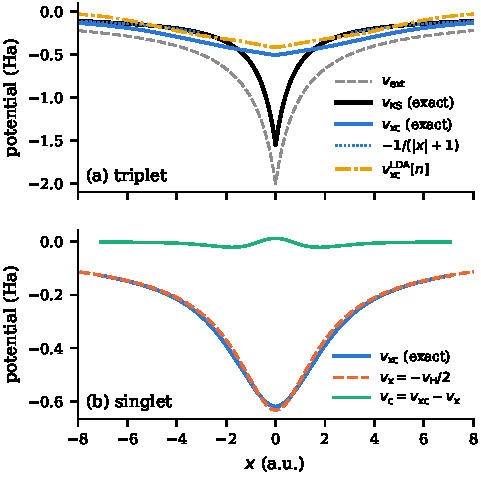
\includegraphics[width=\columnwidth]{figures/fig2_potentials.pdf}
\caption{Exact KS and xc potentials obtained by reverse engineering exact densities of the softened atom of Fig.~\ref{fig:gs}. (a) Spin-polarised (\texttt{uu}) electrons, compared with the LDA xc potential of the same density. (b) Spin-singlet (\texttt{ud}) electrons, for which the exact exchange potential is $-\vH/2$, giving the exact correlation potential $v_\mathrm{c}$. Potentials are shifted to vanish at the left edge of the box.}
\label{fig:ks}
\end{figure}
Reverse engineering the exact density of the spin-polarised atom (Fig.~\ref{fig:ks}a) gives the exact KS potential, and hence $\vxc$. The density of the resulting KS system reproduces the exact density to $\int|n_\mathrm{KS}-n|\,\mathrm{d}x=\numdnRE$. Near the nucleus the exact $\vxc$ and the LDA evaluated on the same density are close. In the low-density tail, however, the LDA decays too quickly: at $x=-8$, where $n\approx\numnTail$, the exact $\vxc$ is $\numvxcTailExact$~Ha but the LDA gives $\numvxcTailLDA$~Ha. The exact potential must decay slowly there to cancel the self-interaction contained in the Hartree potential. For the spin-singlet atom (Fig.~\ref{fig:ks}b, exact energy $\numEsinglet$~Ha) the exact exchange potential of two electrons in one spatial orbital is $-\vH/2$, so reverse engineering isolates the exact correlation potential $v_\mathrm{c}$ directly. The same procedure, applied with other methods in place of the non-interacting solver, gives exact Hartree- or HF-like fictitious systems.

\paragraph{Dynamics}
\begin{figure}[t]
\centering
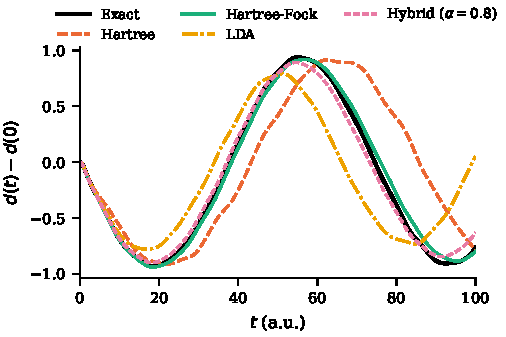
\includegraphics[width=\columnwidth]{figures/fig3_dynamics.pdf}
\caption{Dipole moment $d(t)=\int x\,n(x,t)\,\mathrm{d}x$ of the atom of Fig.~\ref{fig:gs} after a uniform-field pulse of strength $\numtdField$~a.u.\ and duration $\numtdPulse$~a.u., from exact propagation and from the time-dependent Hartree, HF, adiabatic LDA and hybrid methods ($N_x=\numtdNx$, $\numtdSteps$ time steps).}
\label{fig:td}
\end{figure}
Figure~\ref{fig:td} shows the free dipole oscillation of the same atom after a short field pulse. The exact many-body propagation of $\numtdSteps$ steps takes about $\numtdTime$~s on the test machine. The approximate methods are propagated through the same interface. The adiabatic LDA oscillates too fast and time-dependent Hartree theory too slowly, while TDHF and the hybrid follow the exact dipole closely over the first period. The exact time-dependent density can in turn be reverse engineered to give the exact time-dependent KS potential~\cite{Hodgson2013,Hodgson2016}.

% ---------------------------------------------------------------------------
\section{Conclusions}

\iDEA{} provides exact many-electron solutions of 1D model systems, the standard approximate methods and exact reverse engineering of KS and other fictitious-system potentials, ground state and time dependent, behind a single small Python interface. Because the wavefunction is stored on an $N_x^N$ grid, the exact solver is limited in practice to two or three electrons on grids of a few hundred points (Table~\ref{tab:validation}). This is enough for the reference calculations that motivate the code and allows them to run interactively. The simple density-update scheme of Eq.~(\ref{eq:re}) converges reliably for single systems, but it can stall for weakly coupled subsystems, where the KS orbitals are nearly degenerate. More robust inversion algorithms~\cite{Jensen2018,Kanungo2019,Shi2022} are a natural extension. Future directions include symmetry-adapted and tensor-network representations to reach more electrons, and further approximate functionals. \iDEA{} is developed openly, and contributions are welcome.

\section*{Acknowledgements}
We thank all those who have contributed to \iDEA{} and its predecessors, including S.~Adamson, J.~Chapman, T.~Durrant, I.~Edwards, R.~Elmaslmane, M.~Entwistle, F.~Faria, D.~Kooi, P.~Lillystone, A.~Long, S.~Lynn, R.~Oliver, J.~Ramsden, V.~Ravindran, E.~Richardson, P.~Sharp and M.~Smith.

\bibliographystyle{elsarticle-num}
\bibliography{refs}

\end{document}
